%\documentclass[12pt,t]{beamer}
\documentclass[xcolor=svgnames]{beamer}

%\usecolortheme[named=DarkBlue]{structure}

\useoutertheme{infolines}
\usetheme{Boadilla}
%\usetheme[heigth=7mm]{Rochester}
%\usetheme{Rochester}
%\usetheme{Warsaw}
\usecolortheme{whale}


%\setbeamertemplate{blocks}[rounded][shadow=true]
%\setbeamertemplate{navigation symbols}{}
\usepackage[english]{babel}
\usepackage[utf8]{inputenc}
\usepackage{graphicx}
\usepackage{subfigure} 					% uso de many figures


%\usepackage{color}
\usepackage{color, colortbl}
%\usepackage[usenames,dvipsnames,svgnames,table]{xcolor}
\usepackage{xcolor}
\usepackage{booktabs}
\usepackage{comment}
%\usepackage{algorithm2e}
\usepackage{algorithm}
\usepackage{algorithmic}
\usepackage{float}
\usepackage{caption}% http://ctan.org/pkg/caption
%\usepackage{chngcntr}


%\floatname{algorithm}{Procedure}
\renewcommand{\algorithmicrequire}{\textbf{ \colorbox{yellow}{Input:} }}
\renewcommand{\algorithmicensure}{\textbf{  \colorbox{yellow}{Output:} } }
 \definecolor{keywordColor}{RGB}{165, 42, 42}
 \definecolor{componentColor}{RGB}{0, 0, 205}

\renewcommand{\algorithmicfor}{\textcolor[RGB]{165, 42, 42}{\textbf{For}}}
\renewcommand{\algorithmicendfor}{\textcolor[RGB]{165, 42, 42}{\textbf{End}}}
\renewcommand{\algorithmicdo}{\textcolor[RGB]{165, 42, 42}{\textbf{Do}}}
\renewcommand{\algorithmicreturn}{\textcolor[RGB]{165, 42, 42}{\textbf{Return}}}

\newcommand {\otoprule}{\midrule [\heavyrulewidth]}  % This is for getting a bold horizontal line in the 

\bibliographystyle{apalike}
% ------numbering frames-----------------------------------------%
%\newcommand*\oldmacro{}%
%\let\oldmacro\insertshorttitle%
%\renewcommand*\insertshorttitle{%
%	  \oldmacro\hfill%
%	  \insertframenumber\,/\,\inserttotalframenumber
%}
% ---------------------------------------------------------------%

% ------ References ---------------------------------------------%
\usepackage[absolute,overlay]{textpos}
\newenvironment{reference}[2]{%
  \begin{textblock*}{\textwidth}(#1,#2)
      \footnotesize\it\bgroup\color{red!50!black}}{\egroup\end{textblock*}}
% ---------------------------------------------------------------%

%\renewcommand{\figurename}{Figura}
%\renewcommand{\tablename}{Tabela}

% -------------------------------------------------------------- %
% Pacote necessario para subfiguras
\usepackage{multimedia, multirow}
\graphicspath{{./figures/}}
% -------------------------------------------------------------- %



\title[IEEE CAMAD 2012]
    {A Methodology to Define QoS and SLA Requirements in Service Choreographies}
\author[Alfonso Phocco-Diaz]
	{
		{\bf Authors} \\
		Victoriano Alfonso Phocco Diaz \\%\footnote{O aluno recebeu apoio financeiro do CNPq, processo 133147/2009-6} \\ [1ex]
		Daniel Macedo Batista
		%%{\bf Orientador} \\  Daniel Macedo Batista 	\\
		%%{\bf Co-orientador} \\  Marco Dimas Gubitoso 	
	}
\institute[IME-USP]
	{Institute of Mathematics and Statistics \\
	 Departament of Computer Science \\	
	 University of Sao Paulo  \\  [1ex]
	 \texttt{alfonso7@ime.usp.br, batista@ime.usp.br}
	}
\date[September 2012]{September 17, 2012}



%%% Slides ---------------------------------
\begin{document}
%\pgfdeclareimage[width=180pt,height=20pt]{test}{images/header.jpg}
%\logo{\pgfuseimage{test}}


% --- the titlepage frame ------------------------------------------%
\begin{frame}[plain]
  \titlepage
\end{frame}


\section*{Agenda}
    \begin{frame}{Agenda}
        \tableofcontents
    \end{frame}

% ------------------------------------------------------------------%
\AtBeginSection[]
{
	\begin{frame}<beamer>
		\frametitle{}
		\tableofcontents[currentsection]
	\end{frame}
}

% ------------------------------------------------------------------%
% ------------------------------------------------------------------%
% --- Basic Concepts ---------------------------------------------------%
\section{Introduction}

% -----  SOC ----------%
    \begin{frame}{SOC}
       	\begin{block}{SOC (Service Oriented Computing)}\vspace{-.3\baselineskip}
          It  is a new computing paradigm that utilizes services as the basic constructs to support the development
	  of rapid, low-cost and easy composition of distributed applications even in
	  heterogeneous environments.  [Papazoglou et al., 2006]. %\cite{Papazoglou2007}.
        \end{block}
        Key elements:

        \begin{itemize}
           \item <1-> \colorbox{yellow}{Services} (mainly Web services).
           \item <2-> \colorbox{yellow}{SOA}.
           \item <3-> \colorbox{yellow}{Service Composition}.
	    \begin{itemize}
                  \item <4-> \colorbox{yellow}{\textbf{Service Orchestration}}.
                  \item <5-> \colorbox{yellow}{\textbf{Service Choreography}}.
                \end{itemize}
           \item <6->...
        \end{itemize}

    \end{frame}


%----------------- SOA -------------------%
  \begin{frame}{Web Services and SOA}
    	         \only<1>{	
              \begin{figure}[!h]
                  \centering
                  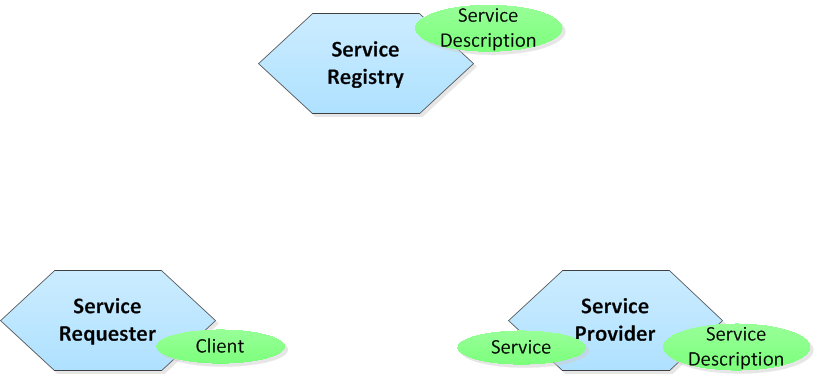
\includegraphics[width=0.9\textwidth]{SOA-Triangle_1.png}
                  \caption{SOA triangle (based on [W3C, 2002])}
              \end{figure}	
          }
          \only<2>{	
              \begin{figure}[!h]
                  \centering
                  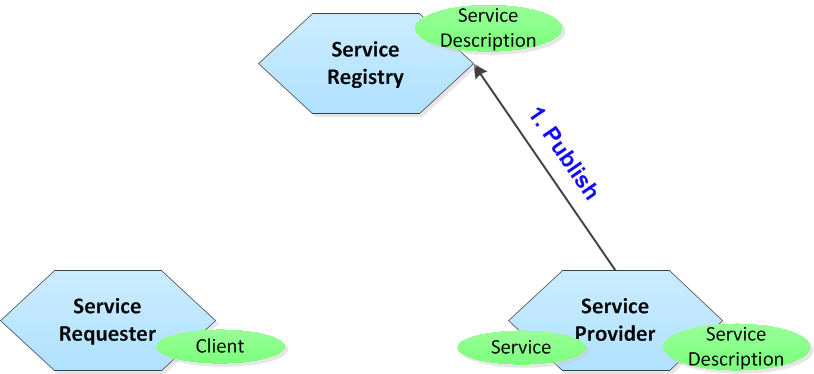
\includegraphics[width=0.9\textwidth]{SOA-Triangle_2.png}
                  \caption{SOA triangle (based on [W3C, 2002])}
              \end{figure}	
          }
          \only<3>{	
              \begin{figure}[!h]
                  \centering
                  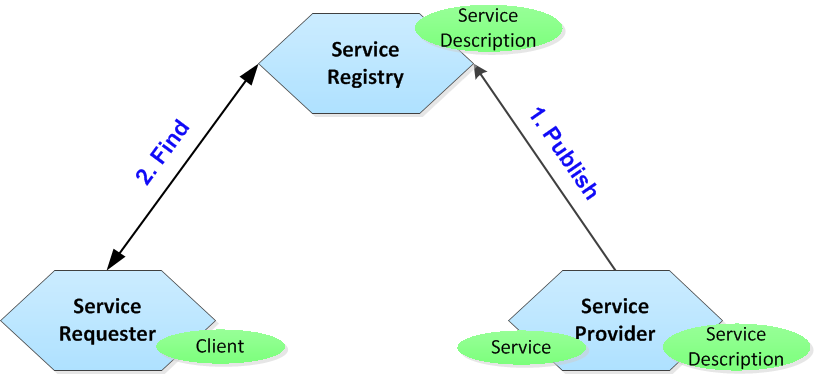
\includegraphics[width=0.9\textwidth]{SOA-Triangle_3.png}
                  \caption{SOA triangle (based on [W3C, 2002])}
              \end{figure}	
          }

          \only<4>{	
              \begin{figure}[!h]
                  \centering
                  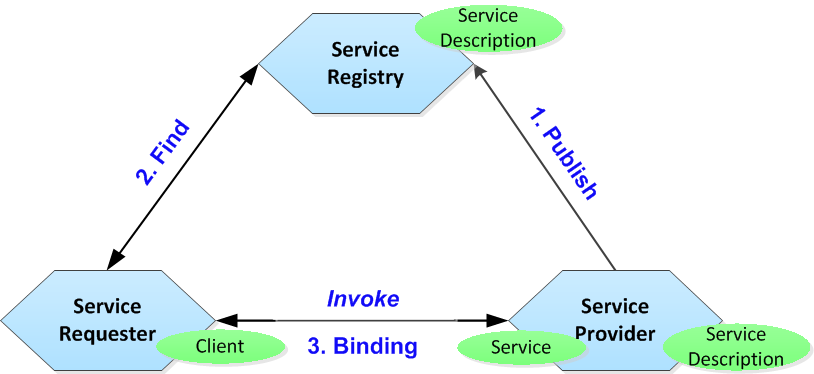
\includegraphics[width=0.9\textwidth]{SOA-Triangle_4.png}
                  \caption{SOA triangle (based on [W3C, 2002])}
              \end{figure}	
          }
          \only<5>{	
              \begin{figure}[!h]
                  \centering
                  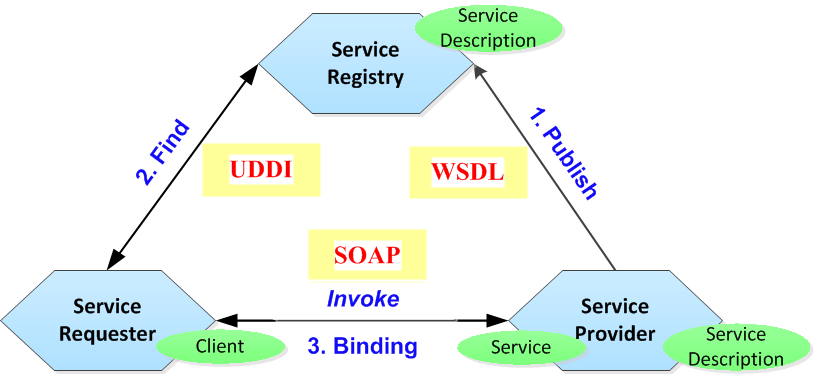
\includegraphics[width=0.9\textwidth]{SOA-Triangle_5.png}
                  \caption{SOA triangle (based on [W3C, 2002])}
              \end{figure}	
          }

    \end{frame}


    %----- Service Orchestration -----%
    \begin{frame}{Service Orchestration}
          \only<1>{	
              \begin{figure}[!h]
                  \centering
                  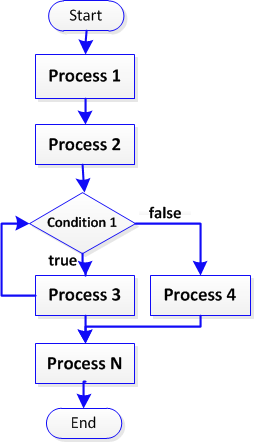
\includegraphics[width=0.25\textwidth]{Orchestration_1.png}
                  \caption{Service Orchestration}
              \end{figure}	
          }
          \only<2>{	
              \begin{figure}[!h]
                  \centering
                  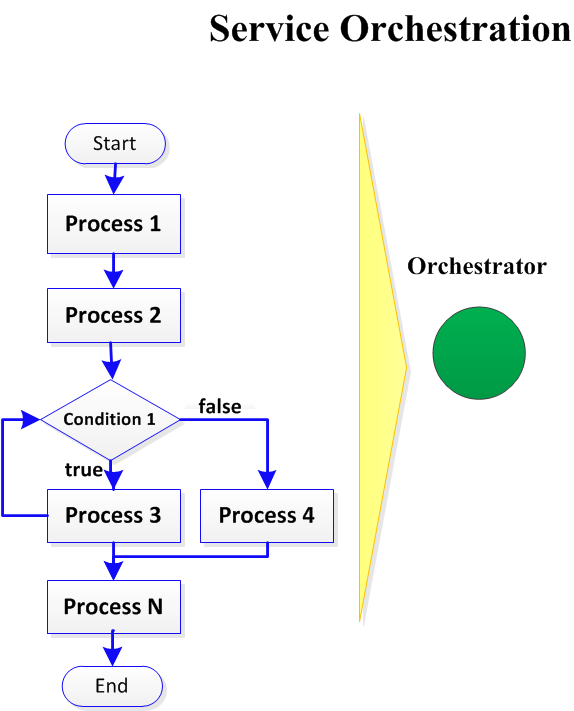
\includegraphics[width=0.45\textwidth]{Orchestration_2.png}
                  \caption{Service Orchestration}
              \end{figure}	
          }
          \only<3>{	
              \begin{figure}[!h]
                  \centering
                  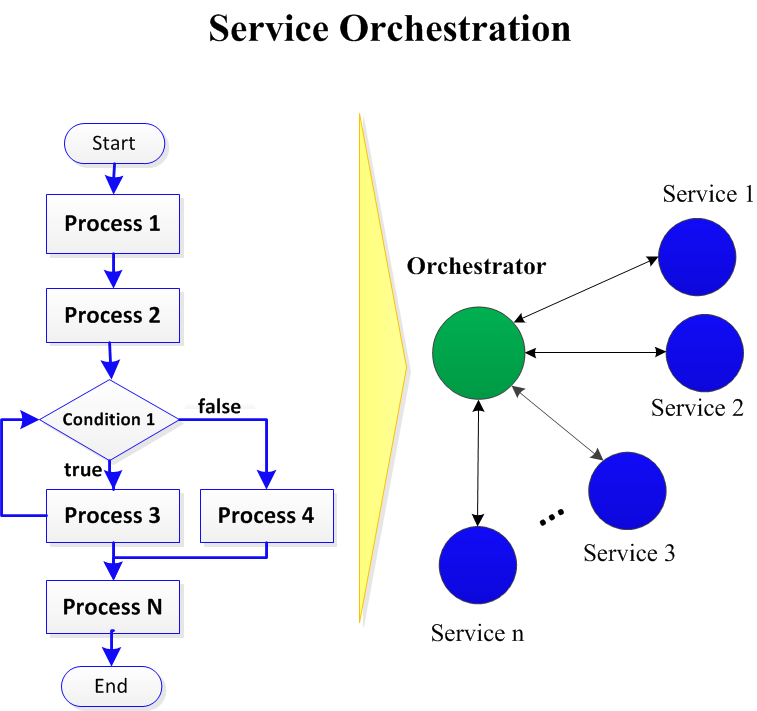
\includegraphics[width=0.5\textwidth]{Orchestration_3.png}
                  \caption{Service Orchestration}
              \end{figure}	
          }

  \end{frame}

    %----- Service Choreography -----%
    \begin{frame}{Service Choreography}
          \only<1>{
	      \begin{itemize}
	        \item Allows service composition in a \textbf{collaborative} manner.
		\item Describes the \textbf{P2P interactions} of the externally \textbf{observable behavior of its participants}.
		\item Don't have a single point of control or coordination.
	      \end{itemize}

	
              \begin{figure}[!h]
                  \centering
                  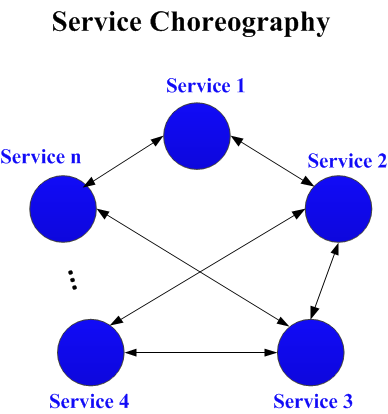
\includegraphics[width=0.4\textwidth]{ChoreographyA.png}
                  \caption{Service Choreography}
              \end{figure}	
          }
          %\only<2>{	
           %   \begin{figure}[!h]
            %      \centering
            %      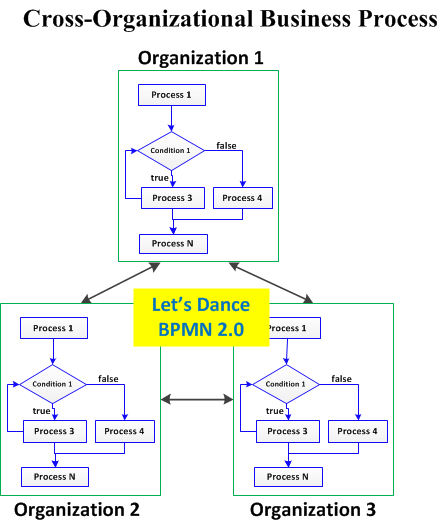
\includegraphics[width=0.6\textwidth]{ChoreographyB_1.png}
            %      \caption{Service Choreography}
            %  \end{figure}	
          %}
          \only<2>{	
              \begin{figure}[!h]
                  \centering
                  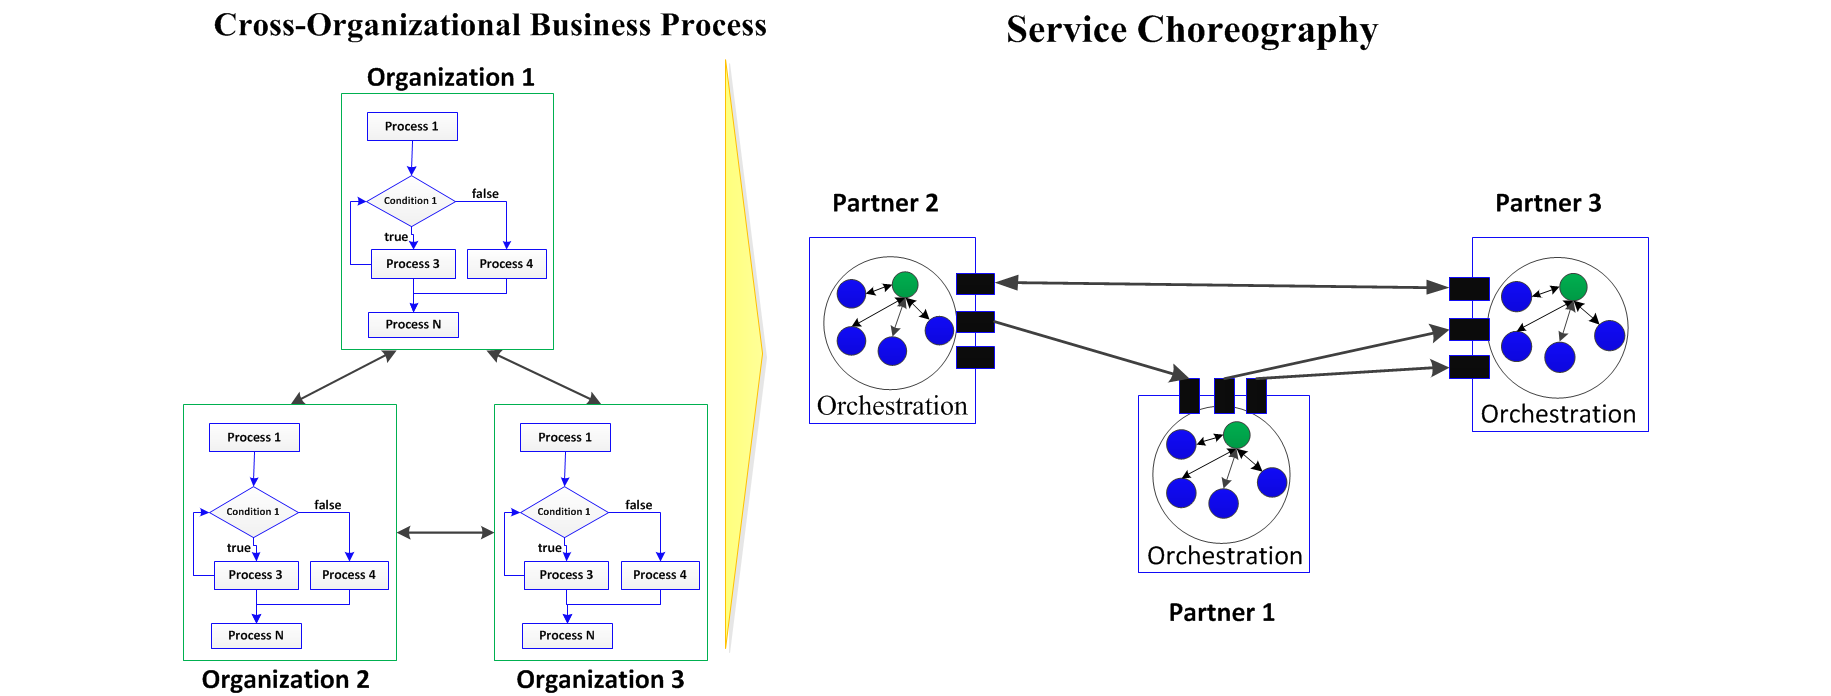
\includegraphics[width=1.0\textwidth]{ChoreographyB_2.png}
                  \caption{Service Choreography}
              \end{figure}	
          }
          \only<3>{
              \begin{figure}[!h]
                  \centering
                  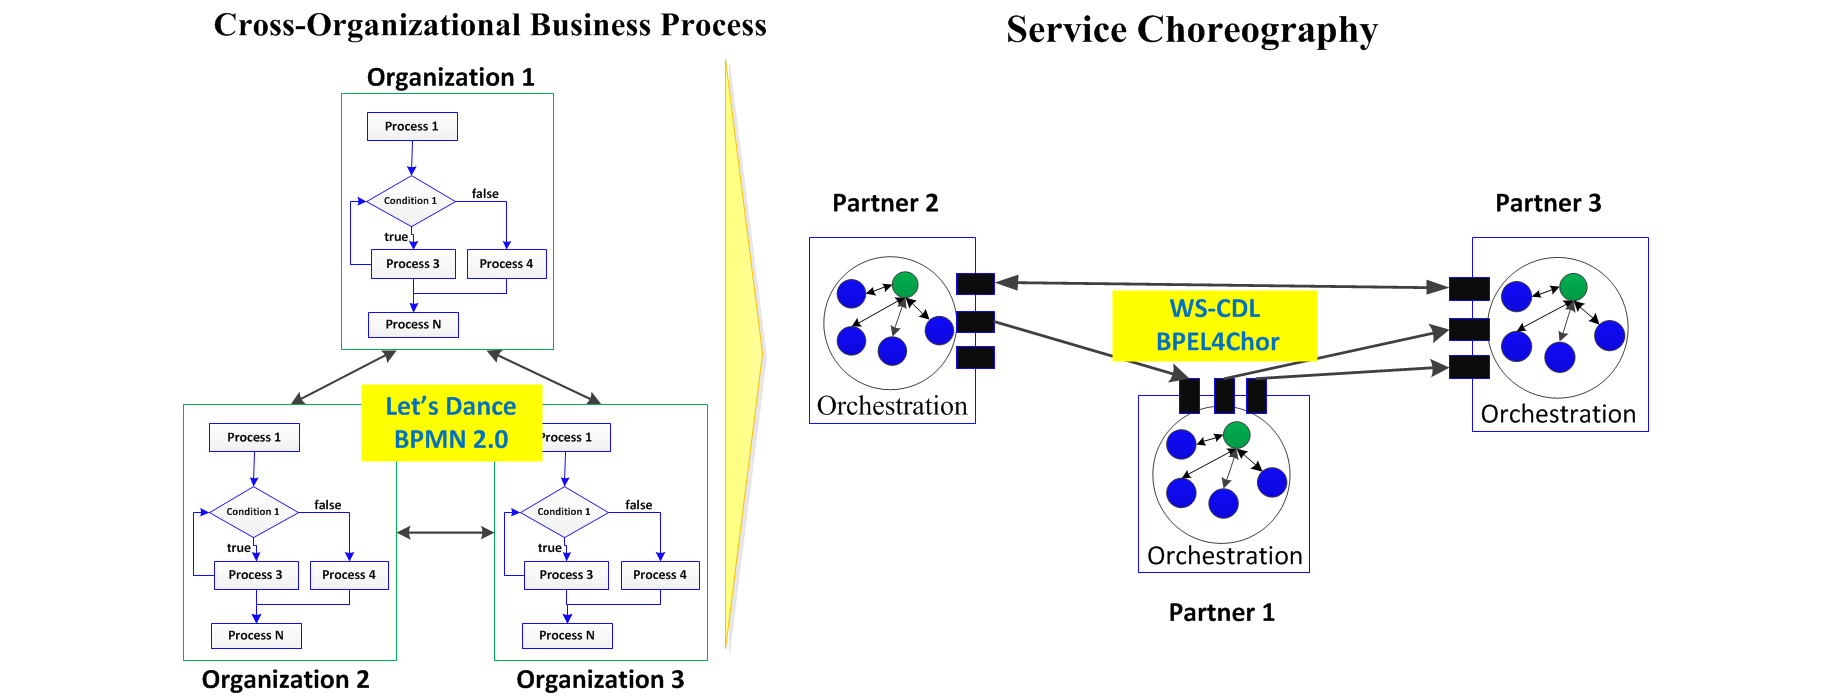
\includegraphics[width=1.0\textwidth]{ChoreographyB_3.png}
                  \caption{Service Choreography}
              \end{figure}
          }
    \end{frame}


%----- QoS -----
%\begin{frame}{Quality of service}



  \begin{frame}{BPMN and Choreography}
    \begin{itemize}
      \item <1-> A Choreography is a type of process.
	\begin{itemize}
	  \item Differs in purpose and behavior from a standard BPMN Process (Process Orchestration).
	  %\item Formalizes the way business \colorbox{yellow}{Participants} \textbf{coordinate} their \colorbox{yellow}{interactions}.
	  \item Formalizes the way business \textcolor{blue}{\textbf{Participants}} \textbf{coordinate} their \textcolor{blue}{\textbf{interactions}}.
	\end{itemize}
      %\item <2-> Focus on the exchange of information (\colorbox{yellow}{Messages}) between these Participants.
      \item <2-> Focus on the exchange of information (\textcolor{blue}{\textbf{Messages}}) between these Participants.
      \item <3-> Two approaches:
	\begin{itemize}
	  \item <4-> \colorbox{yellow}{Interconnection Model}: With collaborations diagrams.
	  \item <5-> \colorbox{yellow}{Interaction Model}:  BPMN Choreographies. using special activities (\textit{Choreography Activity}).
	\end{itemize}
    \end{itemize}

  \end{frame}


  \begin{frame}{Interconnection Model}
      \begin{itemize}
	\item Interconnected public views.	
	\item Use of standard activities.
 	\item ``Collaboration'' in BPMN 2.0.
      \end{itemize}
   \begin{figure}[!h]
	    \centering
	    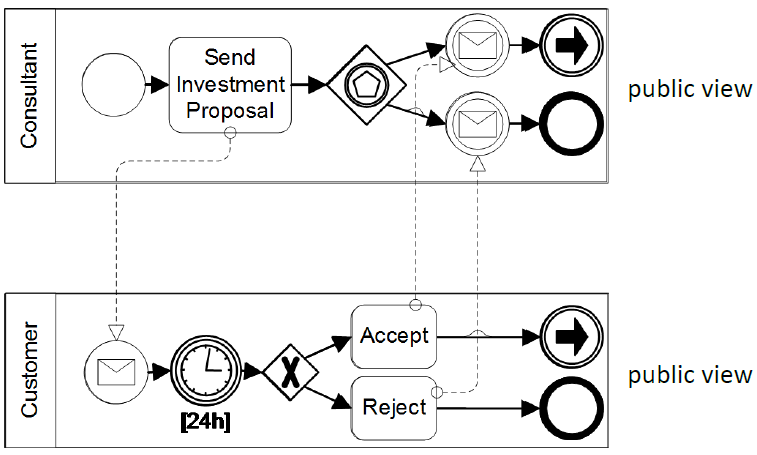
\includegraphics[width=0.8\textwidth]{interconnection_choreography.png}
	    %\caption{BPMN elements for modeling choreographies.}
    \end{figure}	
  \end{frame}


  \begin{frame}{Interaction Model}
    \begin{itemize}
	  \item Interactions \textbf{globally captured}.	
	  \item Basic building block: \textbf{atomic interaction} between two parties.
	  \item ``Choreography'' in BPMN 2.0.
	\end{itemize}
    \begin{figure}[!h]
	      \centering
	      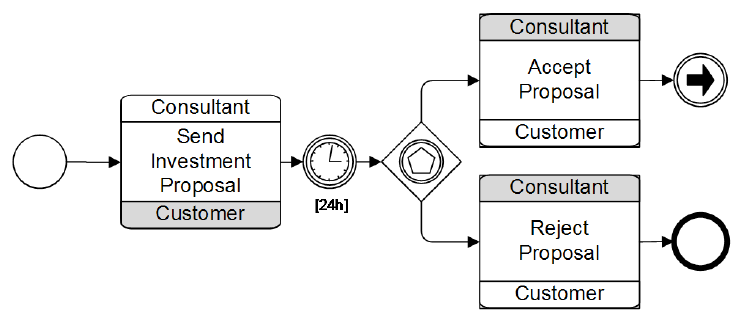
\includegraphics[width=0.8\textwidth]{interaction_choreography.png}
	      %\caption{BPMN elements for modeling choreographies.}
      \end{figure}	
  \end{frame}


  \begin{frame}{BPMN Choreography}

    \begin{figure}[!h]
	      \centering
	      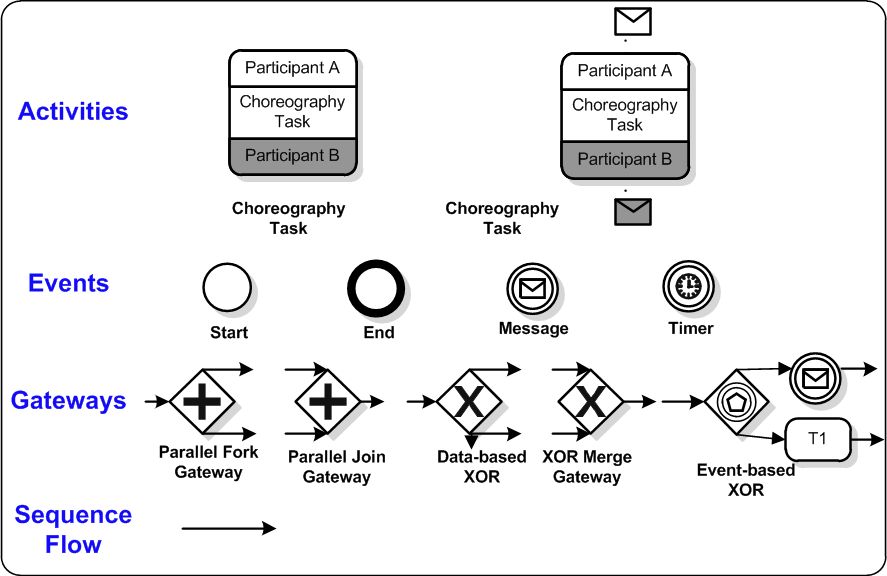
\includegraphics[width=0.8\textwidth]{BPMNBasicChoroegraphy.png}
	      \caption{BPMN elements for modeling choreographies (BPMN 2.0).}
      \end{figure}	
  \end{frame}

  \begin{frame}{ Petri Net (PN)}
      \begin{itemize}
	    \item < 1-> \textbf{PN} is a formalism for modeling \textcolor{blue}{\textbf{concurrency}},  \textcolor{blue}{\textbf{causality}} and \textcolor{blue}{\textbf{conflict}}.	
	    \item < 2-> PN is a \textcolor{blue}{\textbf{bipartite graph}} with the following elements:
  %Petrinetswereintroducedinthe1960sformodellingavarietyof concurrentsystems,buttheiruseforperformancemodelling originatesfrom1980s.
      \end{itemize}

    \only<3>{	
	\begin{figure}[!h]
		  \centering
		  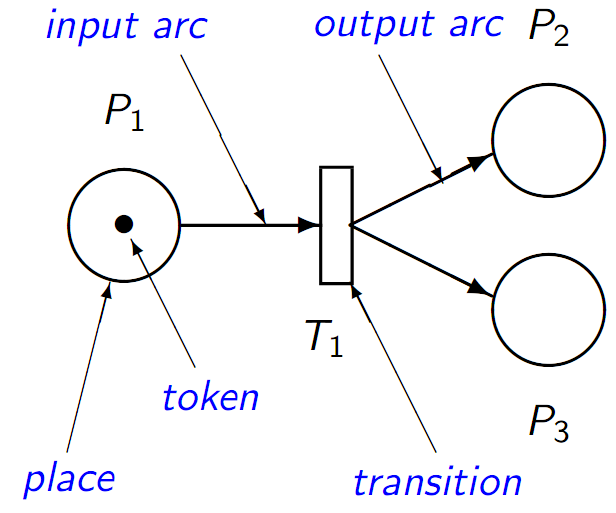
\includegraphics[width=0.4\textwidth]{petrinet.png}
		  \caption{Elements of a petri net.}
	\end{figure}	
    }
  \end{frame}

  \begin{frame}{ Generalized Stochastic Petri Net (GSPN)}
    \begin{itemize}
        \item < 1->\textbf{GSPN} is an extension of PN that associate an \textbf{exponentially distributed delay} with
         the firing of each transition (\textbf{\textcolor{blue}{time transition}}).
        \item < 2->New elements: \textbf{\textcolor{blue}{immediate transitions}}(no time) and \textbf{\textcolor{blue}{inhibitor arcs}}. %and also multiple arcs (inhibitor arcs)
	\end{itemize}

    \only<3>{	
	\begin{figure}[!h]
	      \centering
	      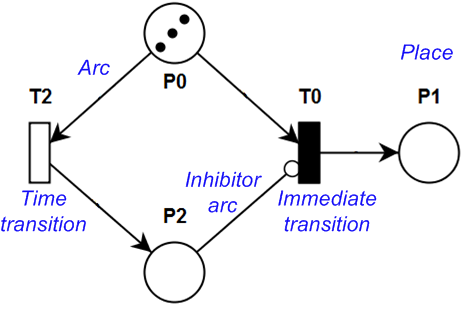
\includegraphics[width=0.5\textwidth]{gspn.png}
	      \caption{Elements of a GSPN.}
	\end{figure}	
    }
  \end{frame}
% ------------------------------------------------------------------%
% ------------------------------------------------------------------%
% ------ Problem ---------------------------------------------------%
\section{Problem}


    \begin{frame}{Problem to Solve}
    	\begin{itemize}
          \item <1-> Planning of resources before/during development of choreography.
          \item <2-> Little approaches don't evaluate choreographies:
	    \begin{itemize}
	      \item focusing on \textbf{QoS} or
	      \item in earlier stages of development.
	    \end{itemize}
          \item <3-> To guarantee QoS about communications (network) is important.
    	\end{itemize}
    \end{frame}

    \begin{frame}
        \begin{block}{Objectives }\vspace{-.3\baselineskip}
        	\begin{itemize}
                  \item To assess the \textbf{impact of QoS} attributes in a \textbf{choreography interaction model}.
		  \item To propose a novel methodology to establish \textbf{requirements for QoS and SLA} in \textbf{early stages of development}.
		  \item To plan the capacity of the network elements in choreographies.
		  \item To convert a interaction model to a GSPN including a QoS model.
            \end{itemize}
        \end{block}
    \end{frame}


\begin{comment}
  \begin{frame}{Justification}
    	\begin{itemize}
          \item <1-> Planning of resources before/during development of choreography.
          \item <2->\textbf{QoS} is a important factor for adaptation, selection, optimization, service composition into SOC.
          plan the capacity of the network elements connecting
the hosts involved in the enactment and deployment of the
choreography.
    	\end{itemize}
  \end{frame}

\end{comment}

% ------------------------------------------------------------------%
% ------------------------------------------------------------------%
% -------------------- Methodology ---------------------------------%
\section{Methodology}
  \begin{frame}{Description}
    \begin{enumerate}
      \item <1-> \textbf{Mapping} of a choreography to a GSPN.
	  \begin{itemize}
	    \item The choreography is specified according ``interaction model''.
	    \item The choreography is specified in BPMN 2.0.
	    \item The resulting GSPN include a QoS model.
	  \end{itemize}

      \item <2-> \textbf{Configurations} of the resulting GSPN.
      \item <3-> \textbf{Simulations} of scenarios.
    \end{enumerate}

  \end{frame}


  \begin{frame}{Choreography Formalization}
    \begin{block}{ Definition: Process Choreography }\vspace{-.3\baselineskip}
      \uncover<1->{A process choreography  is a tuple: }
      \uncover<2->{
         \textcolor{componentColor}{
            \textbf{ $PC = (\mathcal{O, A, E, G, T}, \{e^S\}, \mathcal{E}^I, \{e^E\}, \mathcal{E}^{I_M}, \mathcal{E}^{I_T}, \mathcal{G}^F, \mathcal{G}^J,$
       $\mathcal{G}^X, \mathcal{G}^M, \mathcal{G}^V, \mathcal{F} )$} }where:
        }

      \begin{itemize}
	  \item <2->\textbf{$\mathcal{O}$} is a set of objects and it's partitioned in \textbf{activities $\mathcal{A}$}, \textbf{events $\mathcal{E}$} and \textbf{gateways $\mathcal{G}$}.
	  \item <3-> \textbf{$\mathcal{A}$}, is the set of \textbf{choreography tasks $\mathcal{T}$}.
	  \item <4-> \textbf{$\mathcal{E}$} is the set of \textbf{events} and  it's is partitioned in \textbf{Start event {$e^\mathcal{S}$}}, \textbf{Intermediate
	events $\mathcal{E^I}$} and \textbf{End event {$e^\mathcal{E}$}}.
	  \item <5-> \textbf{$\mathcal{G}$} is the set of \textbf{gateways} and is partitioned in \textbf{parallel fork gateways $\mathcal{G}^F$},
	\textbf{parallel join gateways $\mathcal{G}^J$}, \textbf{data-based XOR gateways $\mathcal{G}^X$}, \textbf{XOR merge gateways $\mathcal{G}^V$} and \textbf{event-based
	XOR gateways $\mathcal{G}^M$}.
	\item <6-> \textbf{$\mathcal{F} \subseteq \mathcal{O}x\mathcal{O}$} is the control flow relation, i.e. a \textbf{set of sequence flows connecting objects}.
      \end{itemize}

    \end{block}

  \end{frame}


  \begin{frame}{QoS Model}
    \begin{itemize} %%Perhaps it's needed use some picture, for example life cycle call service.
	\item Defining the QoS attributes involved in \textbf{service}, \textbf{network} and \textbf{message} aspects.
	\item QoS attributes:
	    \begin{itemize}
	      \item <2->\colorbox{yellow}{In service operation}: \textbf{time to complete the service}.
	      \item <3->\colorbox{yellow}{In network}: delay and \textbf{communication errors}.
	      \item <4->\colorbox{yellow}{In message}: \textbf{message format}.
	    \end{itemize}
    \end{itemize}
  \end{frame}


  \begin{frame}{Mapping BPMN to Petri Net (I)}
    \begin{figure}[!h]
      \centering
      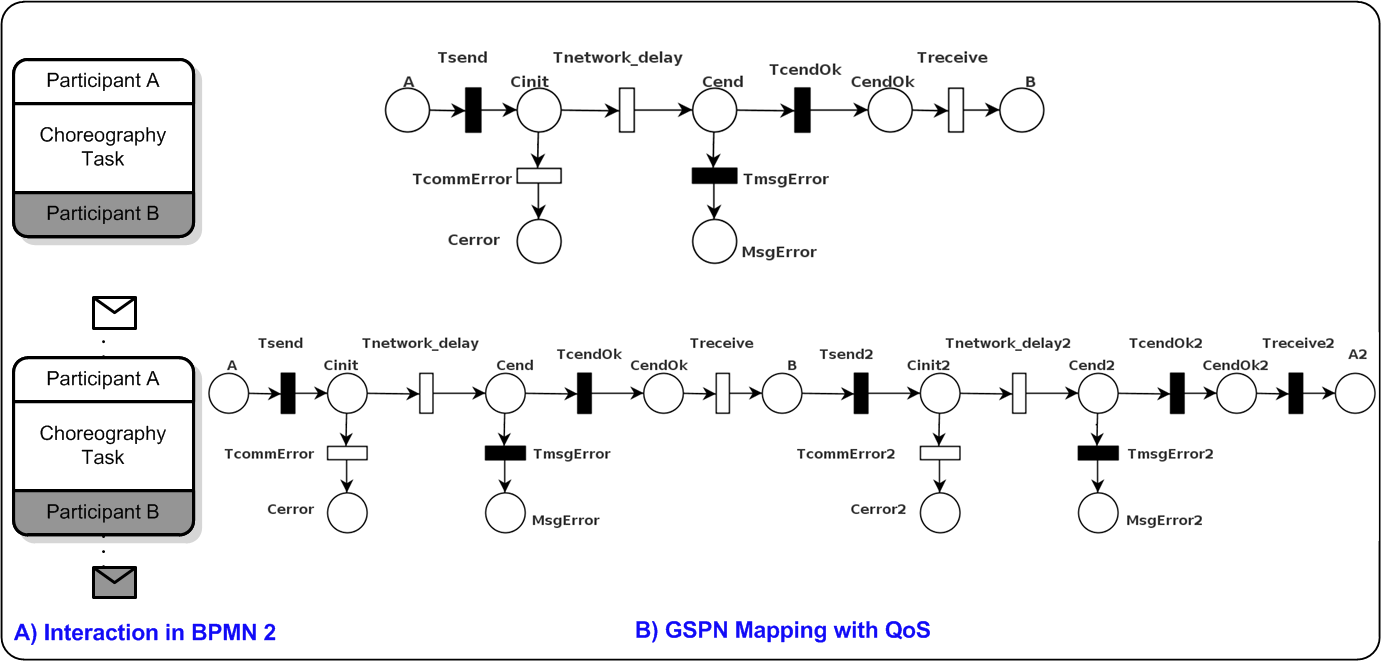
\includegraphics[width=1.0\textwidth]{BPMNChoreographies1-QoS.png}
      \caption{  Mapping of two different choreography tasks with the QoS model}
    \end{figure}
  \end{frame}


  \begin{frame}{Mapping BPMN to Petri Net (II)}
    \begin{figure}[!h]
	\centering
	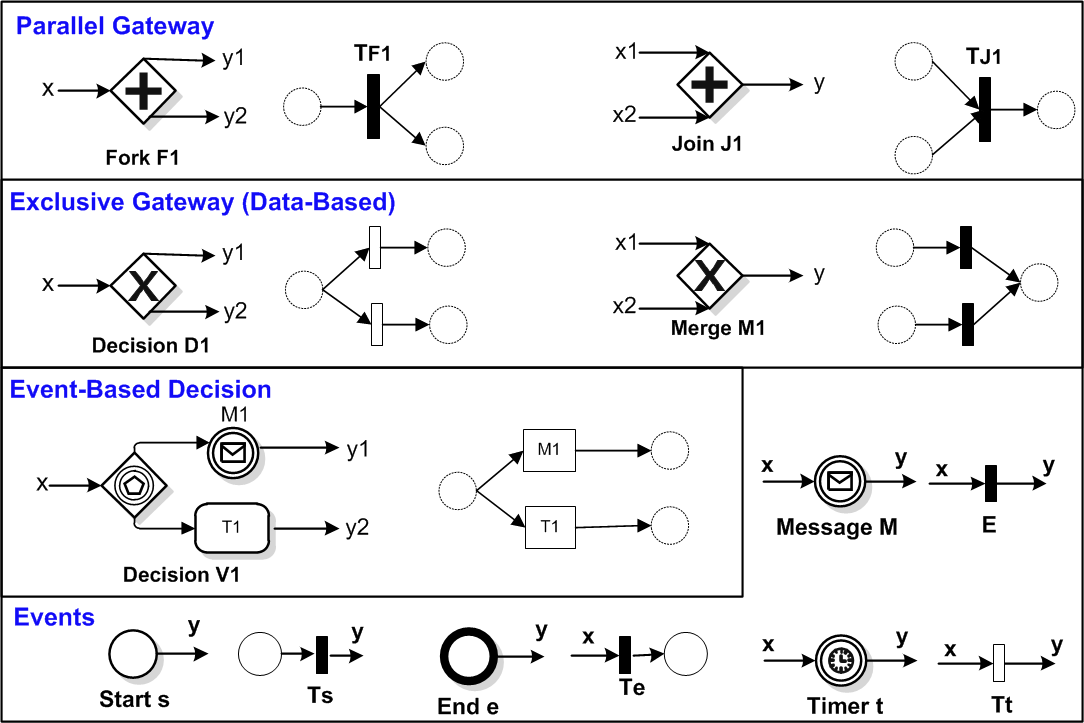
\includegraphics[width=0.95\textwidth]{BPMNChoreographies2_2.png}
	\caption{Mapping of events and gateways elements to modules of Petri nets}
     \end{figure}
  \end{frame}

  \begin{frame}{QoS support}
      \only<1>{	
            \begin{figure}[!h]
            	\centering
            	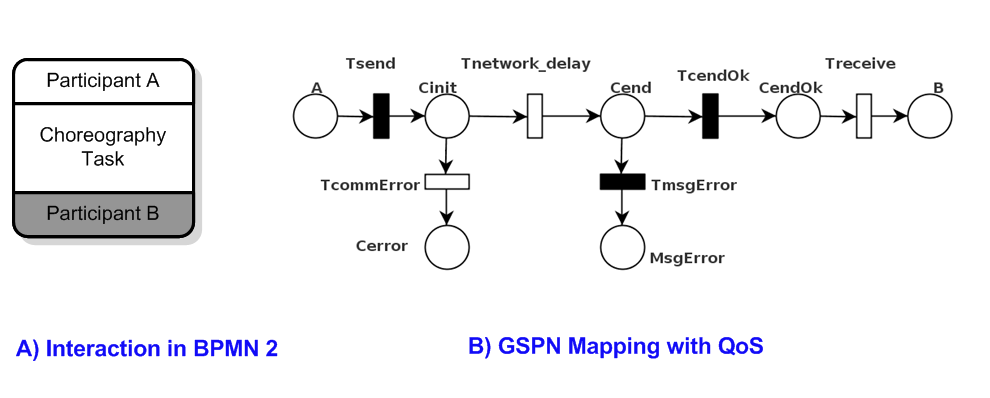
\includegraphics[width=1.0\textwidth]{BPMNTaskChoreography-QoS_Model.png}
            \end{figure}
        }
      \only<2>{	
            \begin{figure}[!h]
            	\centering
            	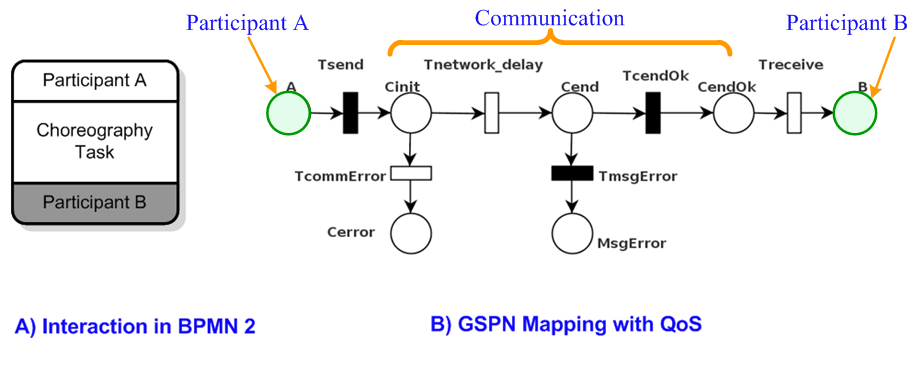
\includegraphics[width=1.0\textwidth]{BPMNTaskChoreography-QoS_Model_1.png}
            \end{figure}
        }
      \only<3>{	
            \begin{figure}[!h]
            	\centering
            	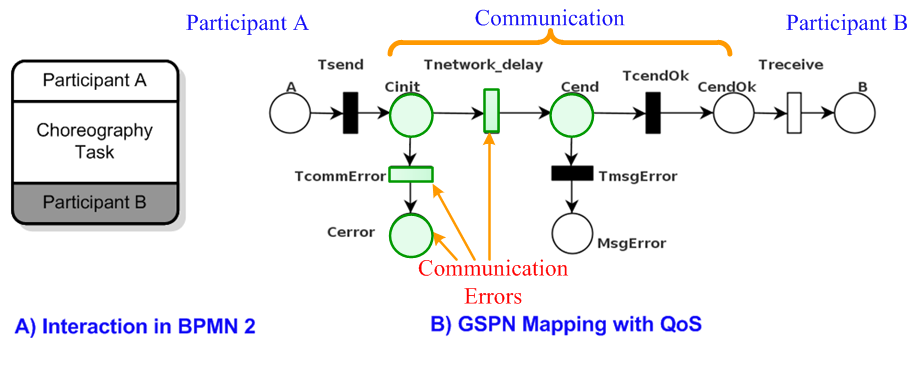
\includegraphics[width=1.0\textwidth]{BPMNTaskChoreography-QoS_Model_2.png}
            \end{figure}
        }
    \only<4>{
            \begin{figure}[!h]
            	\centering
            	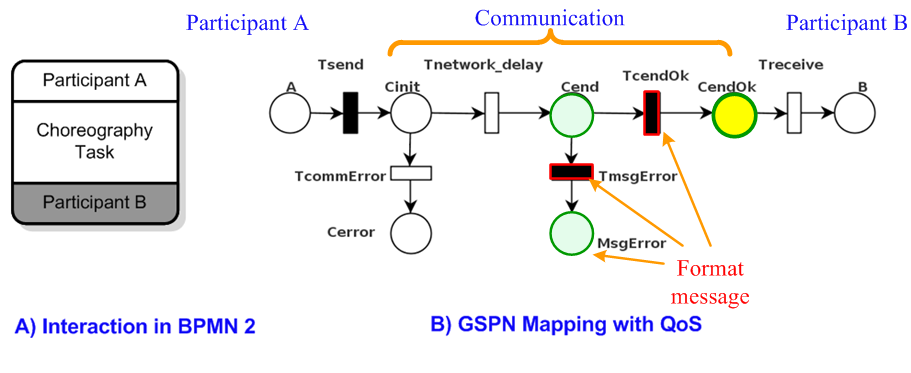
\includegraphics[width=1.0\textwidth]{BPMNTaskChoreography-QoS_Model_3.png}
            \end{figure}
    }
    \only<5>{
            \begin{figure}[!h]
            	\centering
            	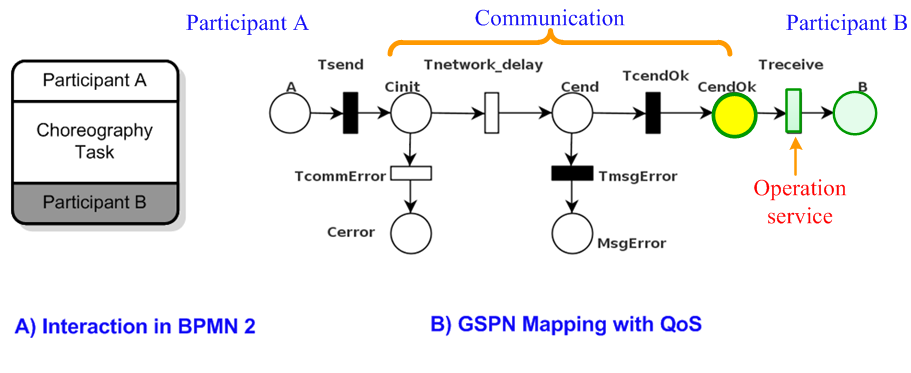
\includegraphics[width=1.0\textwidth]{BPMNTaskChoreography-QoS_Model_4.png}
            \end{figure}
    }
    \only<6>{
            \begin{figure}[!h]
            	\centering
            	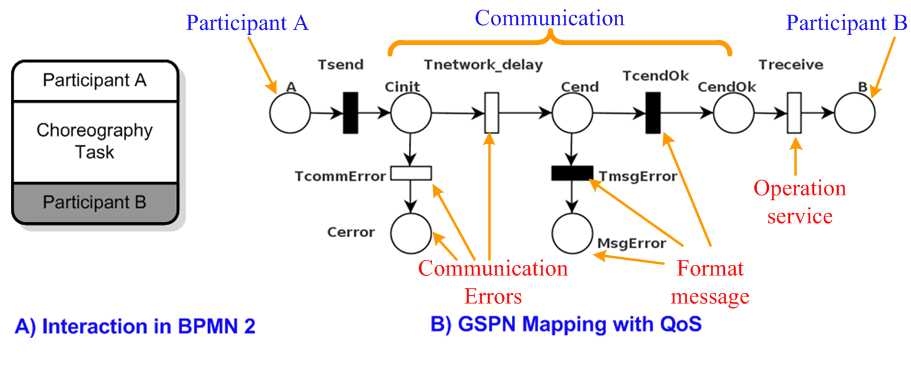
\includegraphics[width=1.0\textwidth]{BPMNTaskChoreography-QoS_Model_5.png}
            \end{figure}
    }
  \end{frame}

%\newcounter{inialg}
%\newcounter{savealg}
%\counterwithout{algorithm}{frame}
  \begin{frame}{Mapping Algorithm (I)}
      \begin{algorithm}[H]

	  %\caption{Mapping a Interconnection Choreography in BPMN onto a GSPN with QoS model}
	    %\caption{ { \small Mapeamento de uma coreografia especificada em BPMN 2.0 para uma GSPN com o modelo de QoS } }
	    \caption*{  \textbf{\textit{Algorithm 1}:}  { \footnotesize     Mapping of choreography specified in BPMN 2.0 to a GSPN with QoS model} }
	    %\label{alg2}
	    \begin{algorithmic}%[1]
	    { \footnotesize
	      %\REQUIRE Process Choreography $\mathcal{PC}$ in BPMN 2.0.
	      \visible<1->{ \REQUIRE \textbf{Process Choreography} \textcolor{componentColor}{ \textbf{ $PC = (\mathcal{O, A, E, G, T}, \{e^S\}, \mathcal{E}^I,$ $\{e^E\}, \mathcal{E}^{I_M}, \mathcal{E}^{I_T},
	      \mathcal{G}^F, \mathcal{G}^J,$ $\mathcal{G}^X, \mathcal{G}^M, \mathcal{G}^V, \mathcal{F} )$} } in BPMN 2.0. }

	    
	      \visible<2->{ \ENSURE Generalized Stochastic Petri Net \textcolor{componentColor}{ \textbf{$GSPN_{QoS}$} }.  }
	
	    \vspace*{3 mm}
	    
	     \visible<3->{ \STATE Consider \textcolor{componentColor}{ \textbf{$CT_i \in \mathcal{T} $, $G_j \in \mathcal{G} $}} and \textcolor{componentColor}{ \textbf{$E_k \in \mathcal{E}$}. where  $i, j, k \in \mathbb{N} $}. }
	      %\STATE Let $PNQoS(CT_i)$ a respective GSPN including QoS from type of $CT_i$ and according to mapping rules (Figure \ref{fig:MappingTaskChoreographiesQoS1}).
	      %\STATE Let $PNQoS(CT_i)$ be a respective GSPN including QoS from type $CT_i$ and according to mapping rules (Figure \ref{fig:MappingTaskChoreographiesQoS1}).
	    \vspace*{3 mm}
	    
	      \visible<4->{ \STATE Consider \textcolor{componentColor}{ $PNQoS(CT_i)$ } is a function of the type of \textcolor{componentColor}{ $CT_i$} that returns a GSPN according to mapping rules. }
	     \visible<5->{ \STATE Consider \textcolor{componentColor}{ $PNQoS(G_j)$ } is a function of the type of \textcolor{componentColor}{$G_j$ } that returns a GSPN according to mapping rules. }
	     \visible<6->{ \STATE Consider \textcolor{componentColor}{ $PNQoS(E_k)$ } is a function of the type of \textcolor{componentColor}{$E_k$} that returns a GSPN according to mapping rules. }
	    \vspace*{3 mm}
	     \visible<7->{ \STATE Consider \textcolor{componentColor}{ \textbf{$\oplus$} } the binary operator of  two GSPNs composition that returns other GSPN. }


	    }
	\end{algorithmic}

      \end{algorithm}

  \end{frame}


%165,42,42
  \begin{frame}{ Mapping Algorithm (II)}


    \begin{algorithm}[H]
	    \caption*{ \textbf{\textit{Algorithm 1}:} { \small   (continued)  }   }
%	    \label{alg2}
	    \begin{algorithmic}
	    { \footnotesize
	
	      \uncover<1->{  \STATE $\textcolor{componentColor}{GSPN_{QoS} } \leftarrow  Empty\  Petri\  Net$  }

	      %\FOR { $CT_i \in T $ }
	      % \STATE $GSPN_{QoS} \leftarrow GSPN_{QoS} \oplus PNQoS(CT_i)$
	      %\ENDFOR

	      \uncover<2->{   \FOR { $\textcolor{componentColor}{ CT_i} \in \textcolor{componentColor}{\mathcal{T}} $ } }
		\uncover<3->{ \STATE $\textcolor{componentColor}{ GSPN_{QoS} } \leftarrow \textcolor{componentColor}{ GSPN_{QoS} } \oplus \textcolor{componentColor}{ PNQoS(CT_i) } $  		}
		\uncover<4->{ \STATE Add a arrival \textbf{timed Transition} at beginning of the \textcolor{componentColor}{$GSPN_{QoS}$}.   }
	     \uncover<2->{  \ENDFOR }
	      \vspace*{3 mm}
	      \uncover<5->{ \FOR{ $\textcolor{componentColor}{G_j} \in \textcolor{componentColor}{\mathcal{G}} $ } 			}
		\uncover<6->{	\STATE $\textcolor{componentColor}{ GSPN_{QoS} } \leftarrow \textcolor{componentColor}{GSPN_{QoS}} \oplus \textcolor{componentColor}{ PN(G_j) }$	}
	      \uncover<5->{ \ENDFOR	}
	    \vspace*{3 mm}
	    \uncover<7->{ \FOR{ $\textcolor{componentColor}{ E_k } \in \textcolor{componentColor}{ \mathcal{E} } $ }					 }	
		\uncover<8->{ \STATE $\textcolor{componentColor}{ GSPN_{QoS} } \leftarrow \textcolor{componentColor}{ GSPN_{QoS} } \oplus \textcolor{componentColor}{ PN(E_k) }$  	}
	      \uncover<7->{ \ENDFOR		}
	      \vspace*{3 mm}
	      \uncover<9->{ \STATE Add a starting Place and \textbf{immediate Transition} at the beginning of the \textcolor{componentColor}{ $GSPN_{QoS}$}.	}
	      \uncover<10->{ \STATE Add a ending Place and \textbf{immediate Transition} at the end of the \textcolor{componentColor}{$GSPN_{QoS}$}.	}
	      \vspace*{3 mm}
	      \uncover<11->{ \RETURN \textcolor{componentColor}{$GSPN_{QoS}$}		}
	    }
	\end{algorithmic}

      \end{algorithm}
  \end{frame}






% ------------------------------------------------------------------%
% ------------------------------------------------------------------%
% -------------------- Performance Evaluation ----------------------%
\section{Performance Evaluation}
  \begin{frame}{Scenario}
      \only<1>{	
            \begin{figure}[!h]
            	\centering
            	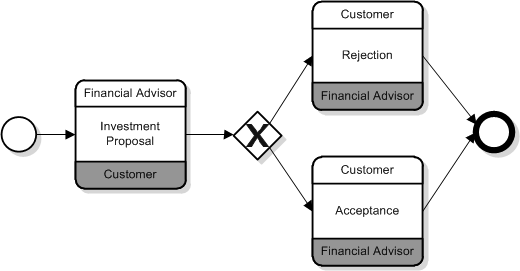
\includegraphics[width=0.85\textwidth]{BPMNChoreographyExample.png}
		\caption{ Choreography example using BPMN2 elements.}
            \end{figure}
        }
      \only<2>{	
            \begin{figure}[!h]
            	\centering
            	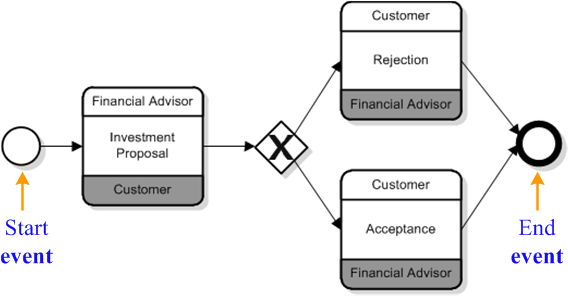
\includegraphics[width=0.85\textwidth]{BPMNChoreographyExample1.png}
		\caption{Choreography example using BPMN2 elements.}
            \end{figure}
        }
      \only<3>{	
            \begin{figure}[!h]
            	\centering
            	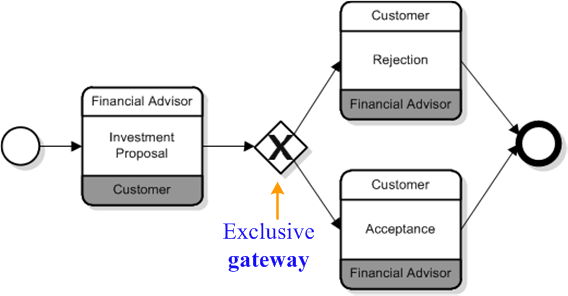
\includegraphics[width=0.85\textwidth]{BPMNChoreographyExample3.png}
		\caption{Choreography example using BPMN2 elements.}
            \end{figure}
        }
      \only<4>{	
            \begin{figure}[!h]
            	\centering
            	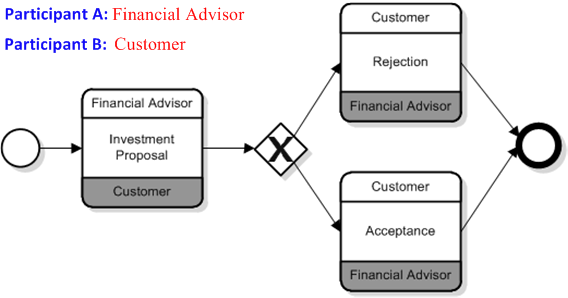
\includegraphics[width=0.85\textwidth]{BPMNChoreographyExample4.png}
		\caption{ Choreography example using BPMN2 elements.}
            \end{figure}
        }
  \end{frame}


  \begin{frame}{Mapping}
    \begin{figure}[!h]
    	\centering
    	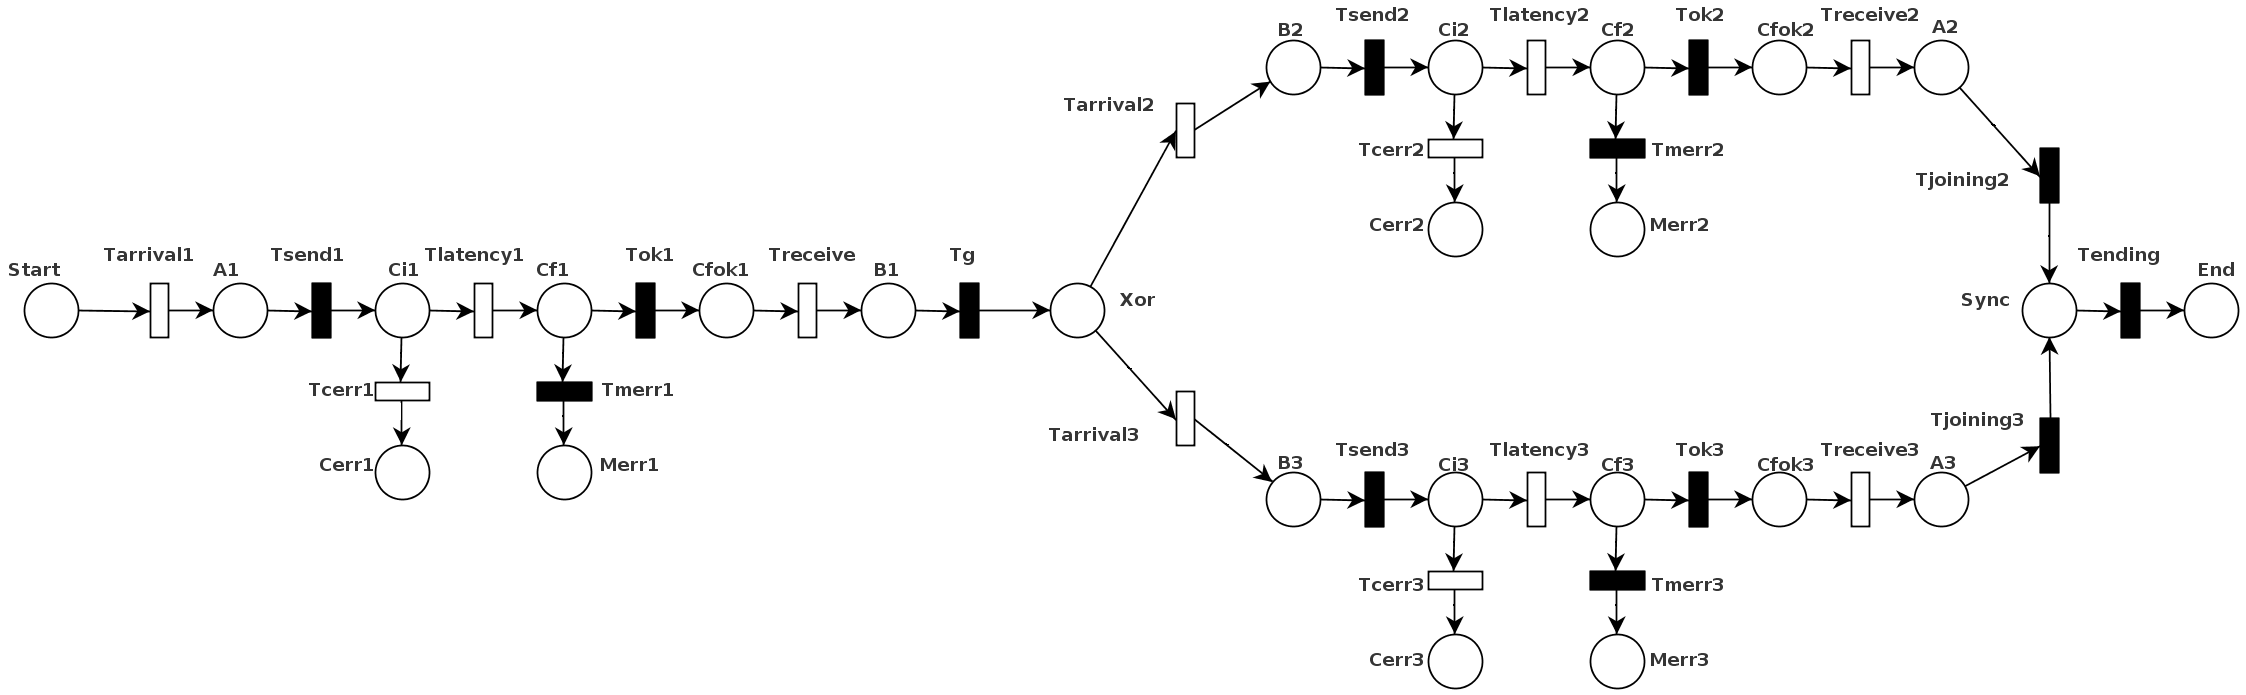
\includegraphics[width=1.0\textwidth]{BPMNChoreographyExample-QoS.png}
    	\caption{GSPN obtained from the choreography.}
    \end{figure}
  \end{frame}


  \begin{frame}{ Configuration (I)}
        \begin{table}[!h]
            \centering
            %\caption{Configuração de pesos nos Cenários 1 e 2}
            \caption{Weights of Scenario 1 and Scenario 2}
            \label{table:transitionsConfigurations}
            \begin{tabular}{ lcc}
              %\cline{1-3}
	      \toprule	
        		    &   \multicolumn{2}{c}{ \textbf{Weights} } \\
              %\cline{1-3}
	      \cmidrule(r){2-3}
              %\hline
              \textbf{Transition}      		&      Scenario 1   &   Scenario 2 		\\
               %\hline
	      \otoprule
               $T_{latency1}$, $T_{latency2}$, $T_{latency3}$ 	& 	0.99       &   0.94	\\
               $T_{cerr1}$, $T_{cerr2}$, $T_{cerr3}$      	&  	0.01 	   &   0.06	\\
               $T_{receive}$, $T_{receive2}$, $T_{receive3}$  &  	99  	   &    97	\\
               $T_{merr1}$, $T_{merr2}$, $T_{merr3}$   &   1 	   &    3	\\
               $T_{arrival2}$, $T_{arrival3}$   &  0.5  &	0.5	\\
              \bottomrule
            \end{tabular}
        \end{table}

  \end{frame}

  \begin{frame}{ Configuration (II)}
    \only<1>{
            \begin{figure}[!h]
            	\centering
            	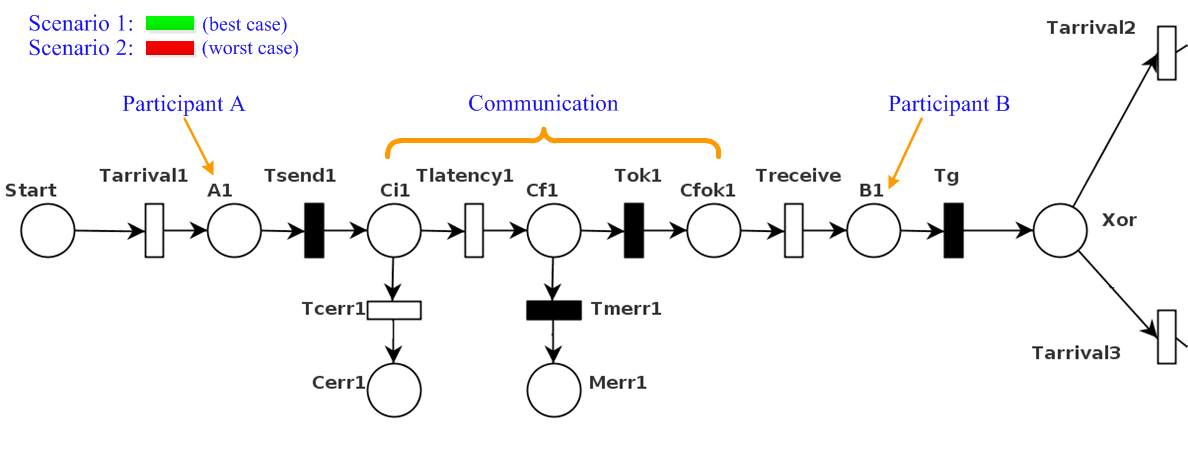
\includegraphics[width=1.0\textwidth]{BPMNChoreographyExample-QoS_configuration1.png}
            \end{figure}
    }
    \only<2>{
            \begin{figure}[!h]
            	\centering
            	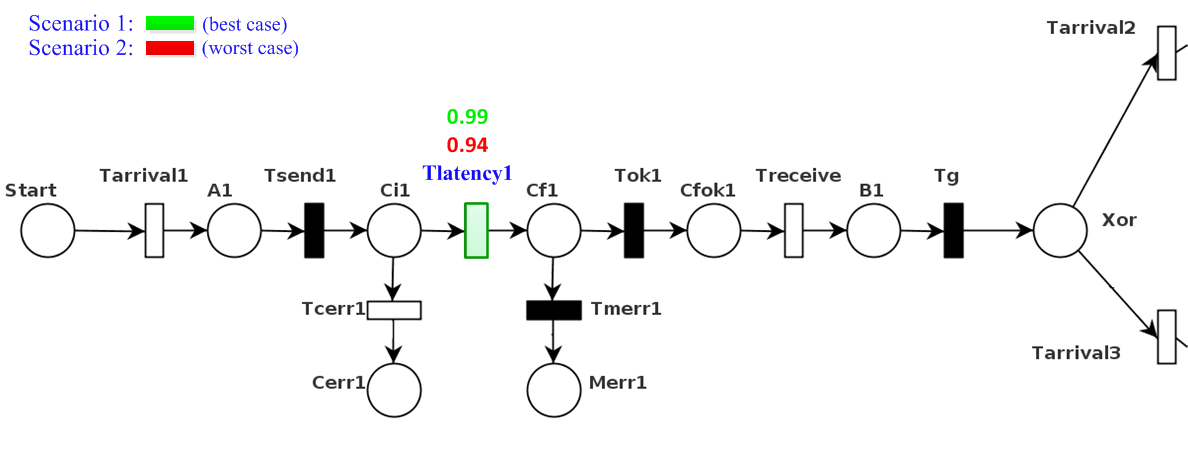
\includegraphics[width=1.0\textwidth]{BPMNChoreographyExample-QoS_configuration2.png}
            \end{figure}
    }
    \only<3>{
            \begin{figure}[!h]
            	\centering
            	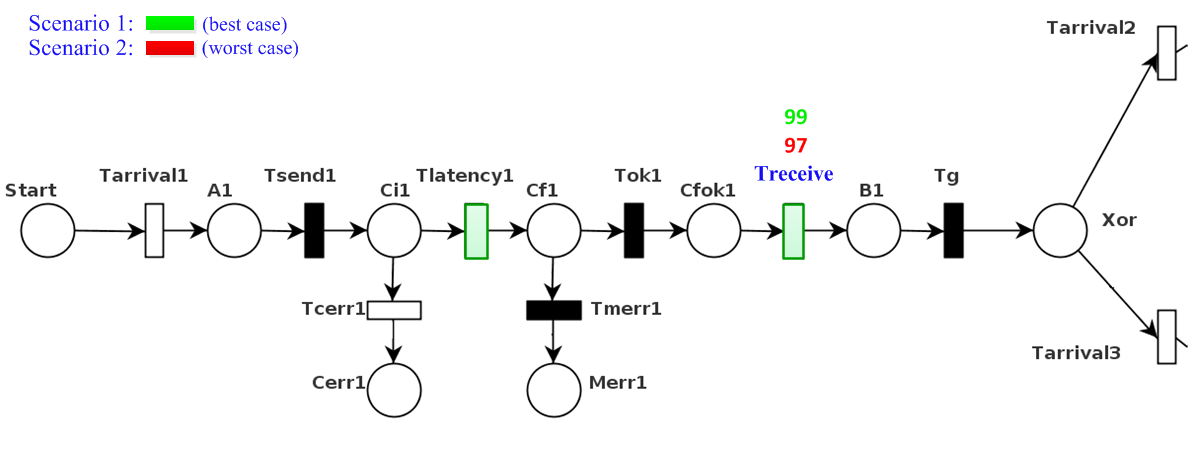
\includegraphics[width=1.0\textwidth]{BPMNChoreographyExample-QoS_configuration3.png}
            \end{figure}
    }
    \only<4>{
            \begin{figure}[!h]
            	\centering
            	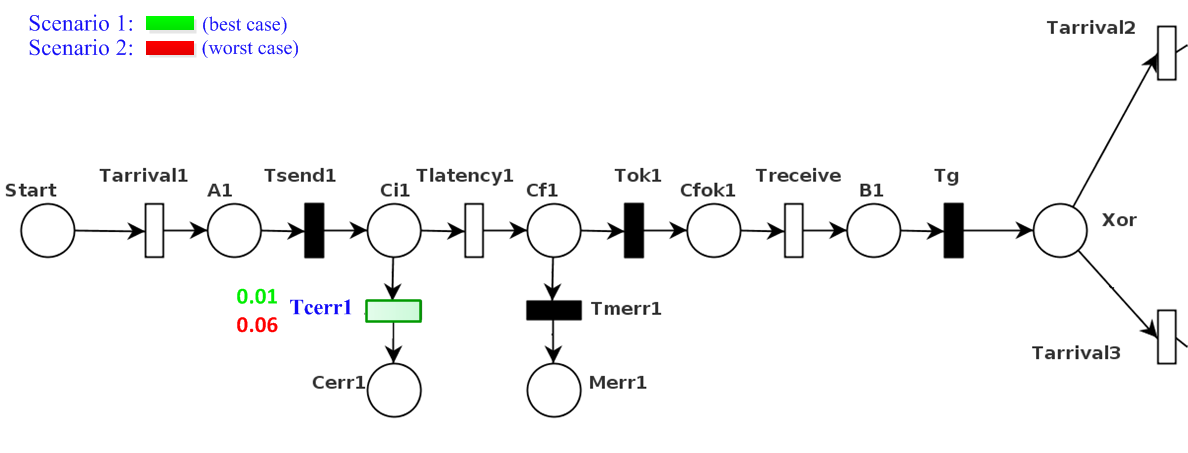
\includegraphics[width=1.0\textwidth]{BPMNChoreographyExample-QoS_configuration4.png}
            \end{figure}
    }
    
  \end{frame}
  
  
  \begin{frame}{ Simulation}
   \begin{itemize}
     \item <1-> \textbf{$1$ token} = \textbf{$1$ choreography instance}.
     \item <2-> \textbf{$100$ tokens} are considered to each scenario at the \textbf{place Start}.
     \item <2-> \textbf{$100$ concurrent instances} were executed (\textbf{multiple-server semantic}).
     \item <3-> The \textbf{Pipe2} tool was used to \textbf{model} and \textbf{simulate} the \textbf{GSPN}.
     \item <4-> $1500$ fires and $10$ replications.
     \item <4-> Confidence level of $95\%$.
   \end{itemize}
  \end{frame}


  \begin{frame}{ Results (I)}

{ \footnotesize
     \begin{table} [tp] %[!h]
            \centering
            \caption{Simulation results } % (in \%) }
            \label{table:simulationsAll}
            \begin{tabular}{l c c c c}
		  \toprule
        	  %\hline
        	 	        & \multicolumn{2}{c|}{ \textbf{Average number of tokens (\%)} } & \multicolumn{2}{c|}{ \textbf{95\% Confidence interval  (+/- \%)} }  \\
        	  %\hline
		  %\cmidrule(r){2-5}
        	  \textbf{Place}      &  Scenario 1   &   Scenario 2  	 &  Scenario 1 	  &   Scenario 2 \\ 
		  \otoprule
		  %\midrule
        	  %\hline
        	  $Start$ &    35.28	 &    40.15        &   5.83    	 &    6.23         \\
        	  $End$   &    41.95	 &    38.78        &   2.53  	  &  3.82	\\
        	  %$A_1$   &    0.08	 &    0.08         &   0.00   	&  0.00     \\ %% após da execucao do Treceive 1
        	  %$B_2$	  &    0.04	&     0.01 		& 	0.01 &  0.01 \\ %% após da execucao do Treceive 2
        	  %$B_3$	  &    0.04	&     0.01  		& 0.01 	&  0.01 \\ %% após da execucao do Treceive 3
              %\hline
		\midrule
        	  %$B_1$	  &    0.08	 &  3.23  		& 0.00	&  0.00	\\ %Primeiro participante em iniciar a interação
        	  %$A_2$	  &    0.04	 &  0.01		& 0.01	&  0.01	\\ %% aceito
        	  %$A_3$	  &    0.04	 &  0.01		& 0.01	&  0.01	\\ %%rejeitado
              %  \hline
        	  $M_{err1}$	& 0.39	 & 0.91 		& 0.95	&  1.92	\\
        	  $M_{err2}$	& 0.00	 & 0.93 		& 0.63		&  0.64	\\
        	  $M_{err3}$	& 0.00   & 0.66 		& 0.87	&  0.74	\\
                %\hline
		\midrule
        	  $C_{err1}$	& 0.74 	 & 2.94 	& 0.82	&  2.02	\\
        	  $C_{err2}$	& 0.00	 & 0.00 	& 0.67	&  1.75	\\
        	  $C_{err3}$ 	& 0.78	 & 0.16 	& 0.92	&  1.52	\\
                %\hline
		\midrule
        	  $C_{i1}$ 	& 8.32	 & 8.90 	& 5.33	&  7.48	\\
              $C_{i2}$ 	& 0.63	 & 0.69 	& 0.23	&  0.52	\\
              $C_{i3}$ 	& 0.75	 & 8.90 	& 0.39	&  0.21	\\

        	  %\hline
		\bottomrule
	  \end{tabular}
        \end{table}
}
  \end{frame}

  \begin{frame}{ Results (II)}
      \begin{itemize}
         \item <1-> \textbf{Communication errors}: An average of  \textcolor{blue}{\textbf{$C_{err1}+C_{err2}+C_{err3}$}} of instances \textbf{didn't finish the process}.
            \begin{itemize}
              \item Scenario 1: \textcolor{blue}{$1.52\%$}.
              \item Scenario 2: \textcolor{blue}{$3.10\%$} (more errors).
            \end{itemize}
         \item <2-> \textbf{Invalid format message}: An average of  \textcolor{blue}{\textbf{$M_{err1}+M_{err2}+M_{err3}$}} of instances \textbf{didn't finish the process}.
            \begin{itemize}
              \item Scenario 1: \textcolor{blue}{$0.39\%$}.
              \item Scenario 2: \textcolor{blue}{$2.50\%$} (more invalid messages).
            \end{itemize}
        \item <3->\textbf{Bottleneck}: It was found a communication bottleneck in the first interaction (\textcolor{blue}{$C_i$} place).
            \begin{itemize}
              \item Scenario 1: \textcolor{blue}{$8.32\%$}.
              \item Scenario 2: \textcolor{blue}{$8.90\%$}.
            \end{itemize}

      \end{itemize}
  \end{frame}




%---------- Conclusions ----------------
\section{Conclusions and Future Works}
   \begin{frame}{Conclusions}
       \begin{itemize}
         \item <1->  We have proposed a Novel methodology to define  QoS and SLA requirements in service Choreography.
         \item <2-> It's a  initial approach using the ``interaction model'' (supported by BPMN $2.0$).
         \item <3-> The GSPN is good to model and analyze several aspects involved into service choreography.
         \item <4-> The simulation is needed for supporting analysis of complex process (e.g. process choreography).
     	 \item <5-> The simulation results can be used to establish early QoS and SLA constraints.
            \begin{itemize}
              \item Integration is expensive, then early detections are needed.
              \item Establishing SLAs according to resources.
              \item Planning in order to reduce failures.
              \item For example: the detected bottleneck can be solved by changing the interaction (modeling issues) or by employing QoS mechanisms in the network to prioritize the traffic affected ( resource planning).
            \end{itemize}
       \end{itemize}
   \end{frame}


  \begin{frame}{Future Works}
       \begin{itemize}
         \item <1-> To extend the mapping to support more choreography BPMN elements.
    	 \item <2-> To expand our methodology to support generic probability distributions in the decision points. Use of Colored Petri Nets (CPNs) can be a alternative.
         \item <3-> To make more analysis and to use complex scenarios, where correlation problems could happen.
         \item <4-> To include more QoS attributes.

       \end{itemize}
   \end{frame}



%\bibliographystyle{apalike}%
%\def\newblock{}
 %       \bibliography{slides}
 %   \end{thebibliography}
%\end{frame}


%--------- fim ----------
    \begin{frame}%{\textbf{Thanks!}}
%        \begin{block}{}\vspace{-.3\baselineskip}
	%\resizebox{dimH}{dimV}{Texto}
	%\resizebox{!}{1cm}{Tamanho}
%	  \begin{center}
%	      {\Huge Thanks!}		            
%	  \end{center}
%        \end{block}

	\begin{beamercolorbox}[sep=2em,wd=10cm]{postit}
	    \begin{center}
	      {\Huge \textbf{\textcolor{blue}{Thanks!}}}		            
	    \end{center}
	\end{beamercolorbox}
	%\mbox{}\medskip\newline

    \end{frame}


\end{document}